\documentclass[11pt]{article}

\usepackage{float}
\usepackage{hyperref}
\usepackage{fullpage}
\usepackage{verbatim}
\usepackage{moreverb}
\usepackage{graphicx}
\usepackage{parskip}
\usepackage{amsmath}
\usepackage[toc,page]{appendix}
\graphicspath{{images/}}

\usepackage{minted}
\let\verbatiminput=\verbatimtabinput
\def\verbatimtabsize{4\relax}

\begin{document}
\title{EE 241B HW2 Writeup}

\author{Vighnesh Iyer}
\date{}
\maketitle

\tableofcontents

\section{Extracting and Simulating a Synthesized Design}
We start with an already placed and routed 4-bit decoder and we go through the flow of extracting parasitics, running LVS, and running SPICE simulations of the extracted schematic.

\subsection{Delay of a Path}
For the path from A[2] to Z[15] rise, what is the delay measured by IC Compiler, SPICE simulation without extracted parasitics, and SPICE simulation with parasitics?

\begin{itemize}
	\item IC Compiler: 0.08215 ns = 82.15 ps
	
	This number was derived from the placed and routed design loaded into ICC and the timing path inspector was used to extract the relevant path and display its delay.
	
	\begin{figure}[H]
		\centerline{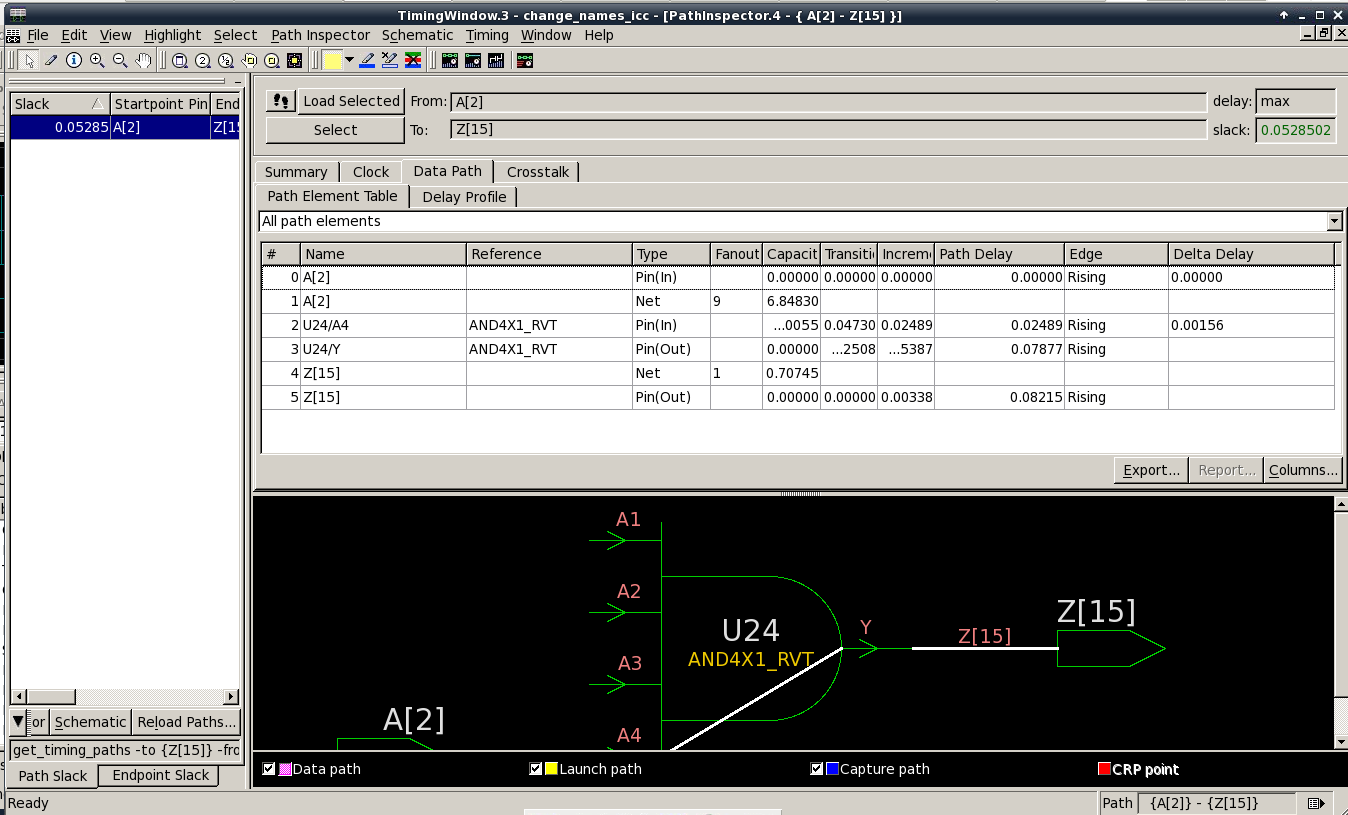
\includegraphics[height=6cm]{icc_path_delay.png}}
	\end{figure}

	\item SPICE without parasitics: 26.297 ps
	
	This number was derived by importing the layout and Verilog netlist into Virtuoso, performing LVS to check that the schematic and layout were representative of the same circuit, and then using the schematic to perform a transistor level SPICE simulation of rising A[2] to rising Z[15].
	
	\begin{figure}[H]
		\centerline{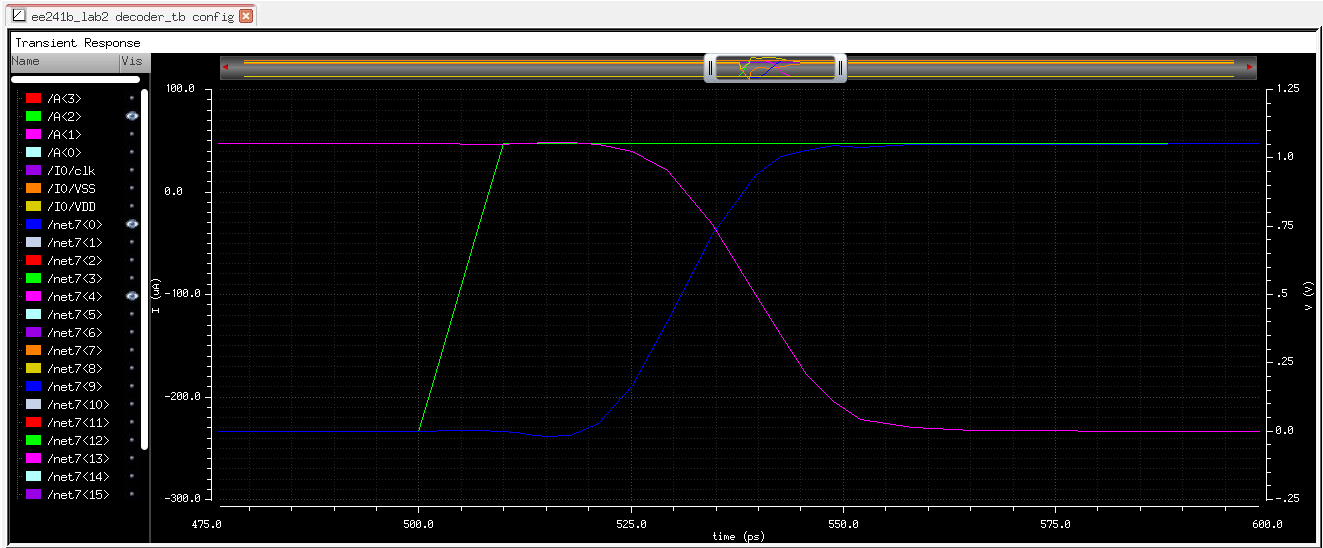
\includegraphics[height=4cm]{spice_path_delay.png}}
	\end{figure}

	In the figure you can see the rise of A[2] (green) followed by the rise of Z[15] (blue) and the fall of Z[11] (pink). The delay in this part is significantly lower than the delay as reported by ICC; it could have to do with parasitics, which will be simulated in the next part.
	
	\item SPICE with parasitics: 46.91 ps
	
	This number was derived using the same testbench, but using the 'starrc' parasitic extracted view of the decoder schematic rather than the raw schematic with ideal circuitry. We can see that the delay increased by almost 2x due to parasitics.
	
	\begin{figure}[H]
		\centerline{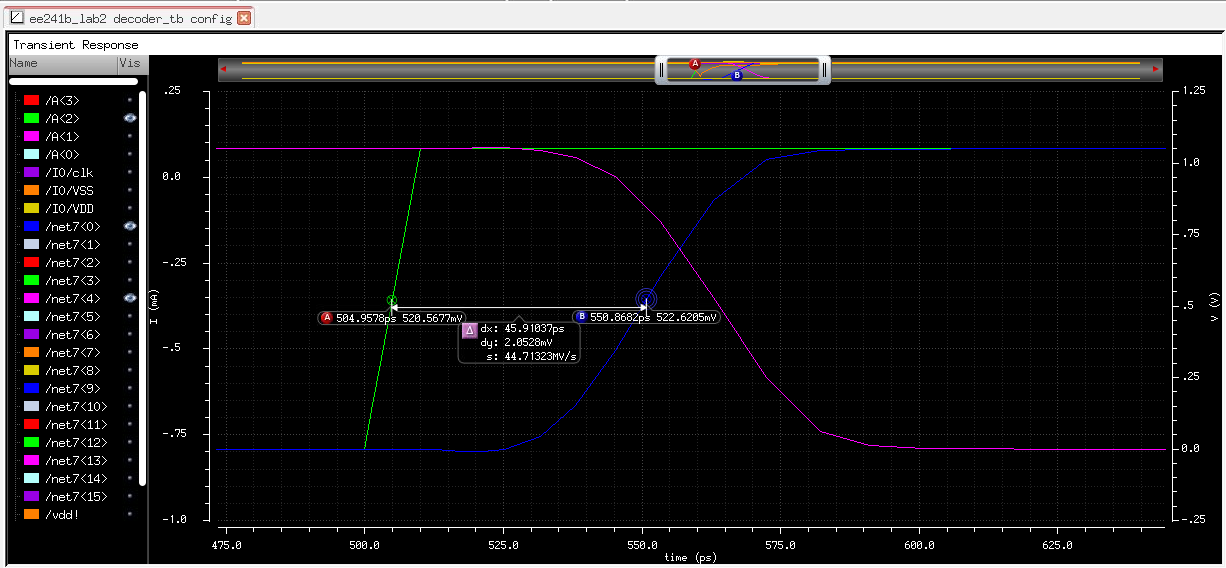
\includegraphics[height=4cm]{spice_path_delay_with_parasitics.png}}
	\end{figure}

	This figure has the same color scheme as the previous one. The path delay is still roughly half of what ICC reported. This probably has to do with some inherent pessimism in the tool.
\end{itemize}

\subsection{ICC Critical Path + Special Path}
We display the critical path in ICC and also highlight the special path noted above from the rise of A[2] to the rise of Z[15].

The critical path is from rising A[3] to falling Z[5], and it has a negative slack of -0.00263 ns. It is highlighted in red. The special path above is highlighted in yellow.

\begin{figure}[H]
	\centerline{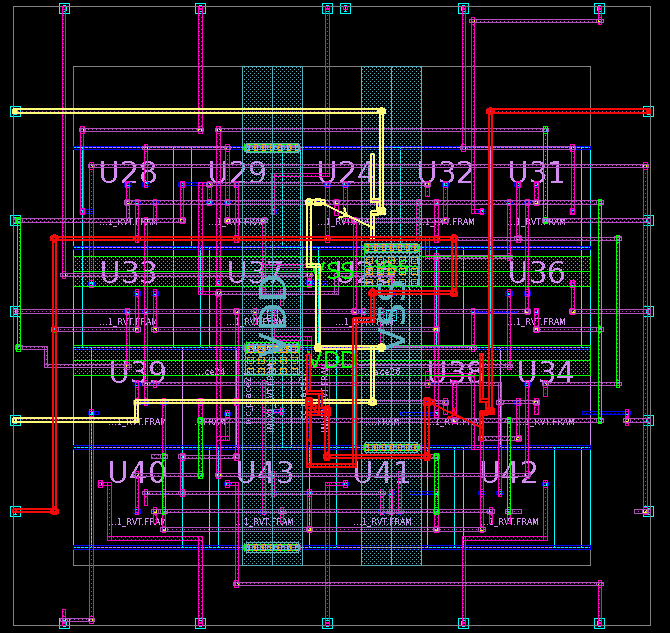
\includegraphics[height=8cm]{icc_critical_path.png}}
\end{figure}

\subsection{Power Estimate Accuracy Analysis}
We run the functional testbench that counts from A=0000 to A=1111 and report the power measured by Primetime, the SPICE simulation, and the mixed-signal simulation.

\begin{itemize}
	\item Primetime: 3.97e-5 (switching), 4.35e-5 (int), 1.90e-6 (leakage), 8.51e-5 (total) = 85 uW
	
	We run a post-PAR simulation using VCS and extract the switching activity SAIF file from the output of the testbench. This file and the Verilog netlist is fed into Primetime which estimates the power usage for the testbench.
	
	\item SPICE: 73.46 uW
	
	We re-create the Verilog testbench in SPICE by using pulsed voltage sources for the \verb|A<3:0>| input to the decoder and we measure the average power consumption by integrating the current drawn from the \verb|VDD| supply during the transient SPICE simulation.
	
	\begin{figure}[H]
		\centerline{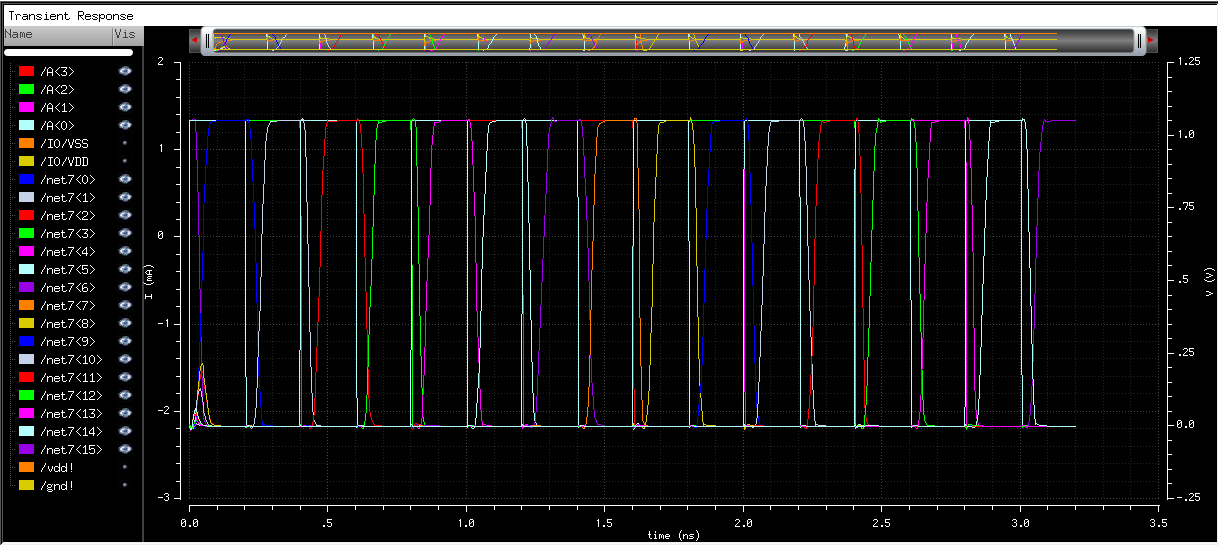
\includegraphics[height=5cm]{spice_power_switching.png}}
	\end{figure}
	
	\begin{figure}[H]
		\centerline{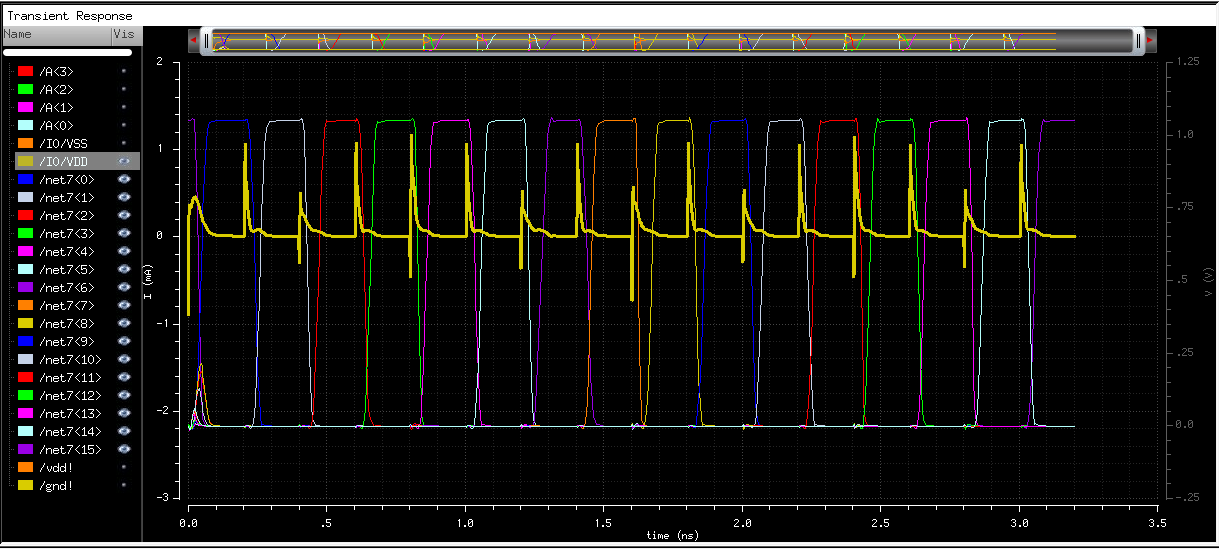
\includegraphics[height=5cm]{spice_power_current_draw.png}}
	\end{figure}

	The first plot shows the switching activity of both the inputs and the outputs of the decoder. The second plot shows the current drawn from the \verb|VDD| input (bold yellow line) of the decoder and each output bit of the decoder going high as its respective code is applied to the decoder's input. The power consumed is measured by using the \verb|average| function on the transient current on the decoder's \verb|VDD| port and multiplying by the supply voltage of 1.05 V.
	
	The power consumed as reported by SPICE with parasitics is a little lower than what was reported by PrimeTime.
	
	\item Mixed-Signal: 75.79 uW
	
	We then set up a mixed-signal testbench by exporting the SPICE netlist of the extracted decoder. We create a wrapper for the decoder in Verilog and instantiate it in a testbench. The testbench is used to drive the inputs and check the outputs of the decoder, while the actual function of the decoder is simulated at the transistor level. This combines the best parts of the Primetime and SPICE flows by letting us write stimulus at a high-level (in Verilog), but still retain the precision of a transistor level simulation using SPICE.
	
	\begin{figure}[H]
		\centerline{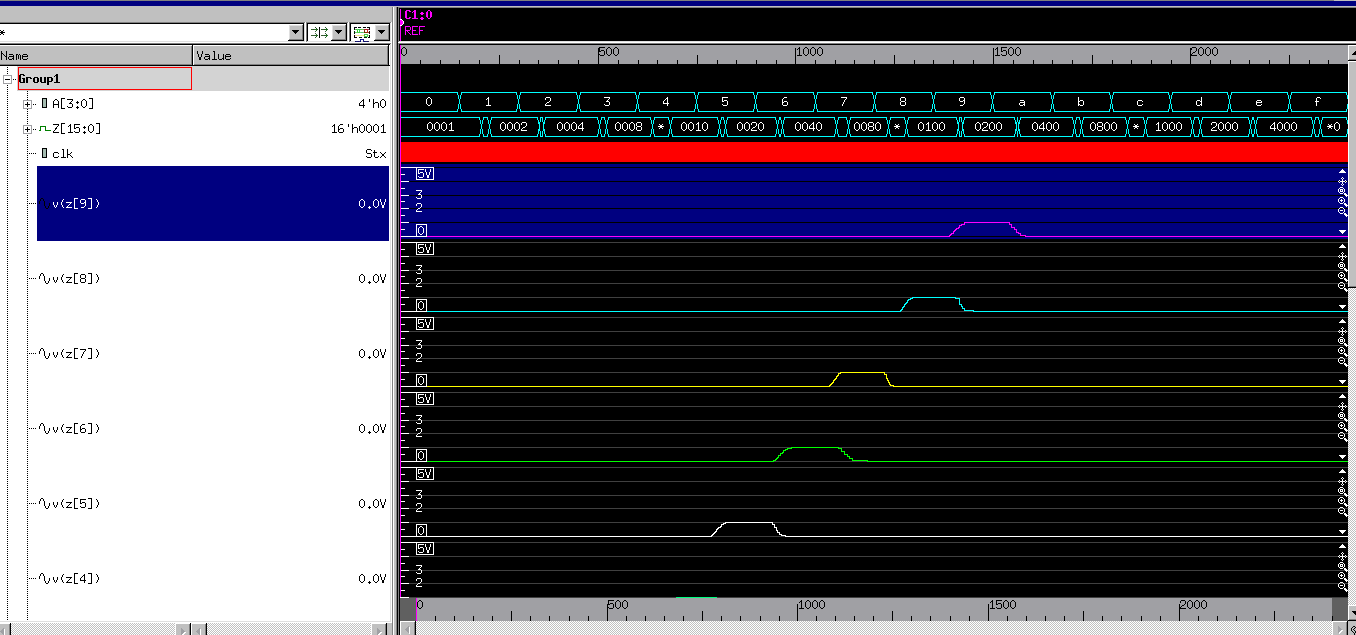
\includegraphics[height=6cm]{mixed_signal_power_analysis.png}}
	\end{figure}

	This snapshot from DVE shows the digital stimulus applied to the decoder and the SPICE simulated decoder's analog outputs.
\end{itemize}

\subsection{Voltage Scaling Power Estimates}
We run the mixed-signal simulation at 1.05V, 0.8V, 0.6V, and 0.4V and measure the average power for each voltage. We then convert average power to energy/op in terms of J/op and uW/Mhz. These results are compared to the theoretically predicted active energy savings for voltage scaling based on the 1.05V result.

The clock period will have to increase for lower supply voltages to compensate for increased delay.

\section{FF and Latch Based Timing}

\section{Variability and Timing Simulations}

\newpage
\appendix
\section{PMOS/NMOS DC Characterization SPICE Sim} \label{dc_characterization_spice}


\end{document}